\documentclass[11pt]{article}
\usepackage{scilabrpt}
\usepackage{listings}
\usepackage{color}
\usepackage{subcaption}

\definecolor{mygreen}{rgb}{0,0.6,0}
\definecolor{mygray}{rgb}{0.5,0.5,0.5}
\definecolor{mymauve}{rgb}{0.58,0,0.82}

\lstset{ %
  backgroundcolor=\color{white},   % choose the background color; you must add \usepackage{color} or \usepackage{xcolor}
  basicstyle=\tiny,        % the size of the fonts that are used for the code
  breakatwhitespace=false,         % sets if automatic breaks should only happen at whitespace
  breaklines=true,                 % sets automatic line breaking
  captionpos=b,                    % sets the caption-position to bottom
  commentstyle=\color{mygreen},    % comment style
  deletekeywords={...},            % if you want to delete keywords from the given language
  escapeinside={\%*}{*)},          % if you want to add LaTeX within your code
  extendedchars=true,              % lets you use non-ASCII characters; for 8-bits encodings only, does not work with UTF-8
  frame=single,	                   % adds a frame around the code
  keepspaces=true,                 % keeps spaces in text, useful for keeping indentation of code (possibly needs columns=flexible)
  keywordstyle=\color{blue},       % keyword style
  language=Python,                 % the language of the code
  otherkeywords={*,...},           % if you want to add more keywords to the set
  numbers=left,                    % where to put the line-numbers; possible values are (none, left, right)
  numbersep=5pt,                   % how far the line-numbers are from the code
  numberstyle=\tiny\color{mygray}, % the style that is used for the line-numbers
  rulecolor=\color{black},         % if not set, the frame-color may be changed on line-breaks within not-black text (e.g. comments (green here))
  showspaces=false,                % show spaces everywhere adding particular underscores; it overrides 'showstringspaces'
  showstringspaces=false,          % underline spaces within strings only
  showtabs=false,                  % show tabs within strings adding particular underscores
  stepnumber=2,                    % the step between two line-numbers. If it's 1, each line will be numbered
  stringstyle=\color{mymauve},     % string literal style
  tabsize=2,	                   % sets default tabsize to 2 spaces
  title=\lstname                   % show the filename of files included with \lstinputlisting; also try caption instead of title
}

%%%%%%%%%%%%%%%%%%%%%%%%%%%%
%%%    Begin Document    %%%
%%%%%%%%%%%%%%%%%%%%%%%%%%%%
\begin{document}

\pagenumbering{roman}

\waterlootitle{PHYS 375 Final Project}{
  PHYS 375\\
  %Group
  Waterloo, Ontario\\
  %City 
  }{
  Robert Burnet \\
  3B Physics and Astronomy \\
  ID 20465122\\
  \today
  }


\dotableofcontents

\pagenumbering{arabic}
\section{Algorithmic Choices}
\subsection{Adaptive Runge-Kutta-Fehlberg and Bisection Method}
To solve the stellar structure equations, our group decided to adapt a 4th-5th order adaptive step-sized Runge-Kutta-Fehlberg (RKF45) method (see rkf.py in the \textbf{Appendix}). RKF45 is a numerical method to solve differential equations of order O(h$^4$), using the O(h$^5$) order to estimate error for implementing adaptive step sizes. It is identified by its Butcher Tableau which details the coefficients used for the integration method (see table 1 below).

\begin{table}[h]
\begin{center}
\begin{tabular}{c | c c c c c c}
0 &  & & & & & \\
1/4 & 1/4 & & & & & \\
3/8 & 3/32 & 9/32 & & & & \\
12/13 & 1932/2197 & -7200/2197 & 7296/2197 & & & \\
1 & 439/216 & -8 & 3680/513 & -845/4104 & & \\
1/2 & -8/27 & 2 & -3544/2565 & 1859/4104 & -11/40 & \\
\hline
 & 16/135 & 0 & 6656/12825 & 28561/56430 & -9/50 & 2/55 \\
 & 25/216 & 0 & 1408/2565 & 2197/4104 & -1/5 & 0 \\
\end{tabular}
\caption{Butcher tableau of RKF45}
\end{center}
\end{table}

The numbers to the right of the vertical line and above the horizontal line correspond to elements of the Runge-Kutta matrix, the numbers to the left of the vertical line correspond to the nodes, and the numbers below the horizontal line correspond to the weights. The first row below the horizontal line gives the O(h$^5$) order accurate method where as the second row gives the O(h$^4$) order accurate method \cite{DE}. We use the 5th order to find the error with our step size and adaptively change its size to accommodate for the error. This saves time for solving the differential equations over just carrying out an RK4 method to solve it by allowing us to adaptively change the step sizes as we won't needlessly be using small steps when not much is changing; we can make the step sizes bigger when the solutions to the differential equations don't change as much, and decrease the step sizes only when we need to using this method.

Along with using RKF45 to solve the differential equations, we also employed a type of adaptive bisection method to find the root to the equation:
\begin{equation}
f(\rho_c) = \frac{L_* - 4 \pi \sigma R_*^2 T_*^4}{\sqrt{4 \pi \sigma R_*^2 T_*^4 L_*}}
\end{equation} \label{f_rho}

This bisection method is similar to the one suggested in the project description \cite{manual}, except that it adaptively changes its precision to save time (see adaptive\_bisection.py in the \textbf{Appendix}). At first, all one needs to start the bisection method is a value greater than the desired value, and a value less than the desired value. The precision of the chosen values is not important. The precision only becomes important as you approach the desired value. This method adaptively increases the precision as you approach the desired value, while starting off at a very low precision, all to save time. 

We start with a $\rho_c$ that gives a value of $f(\rho_c)$ greater than 0, and a $\rho_c$ that gives a value of $f(\rho_c)$ less than zero, to a low precision. We then employ bisection method, increase the precision, and carry it out again until we reach a $\rho_c$ that gives $f(\rho_c)$ = 0 to an acceptable precision.

\newpage

\subsection{Creating and Plotting Stars}

stellar\_generator.py details all the differential equations and parameters we needed to solve to create a star. In it, there is a Star class which contains all the parameters, functions, and differential equations needed to solve for the stellar structure equations. It is in here we employ the RKF45 method and adaptive bisection method to solve for the stellar structure. One can call the desired parameters of a solved star by calling its specific attribute from its Star class. For instance, if you wish to attain the central density of the star, you simply call [solved star's variable name].density\_c after solving the star using [solved star's variable name].solve .

stellar\_plotter.py calls stellar\_generator.py with an input star's free parameters (central temperature and X, Y, and Z composition values) to solve the stellar structure equations for that star, and then plots them into the various plots we desire, such as the normalized $\rho$, $T$, $M$, $L$, $P$, $dL/dr$, and $\kappa$ as functions of $r/R_*$ plots, the partial pressures, luminosities, opacities, and the dlogP/dlogT plots. stellar\_plotter.py can also call main\_sequence.py to generate the various main sequence plots.

main\_sequence.py details a MainSequence class which solves the stellar structure equations of various stars, given the range of central temperature, the compositions, and the number of stars desired to generate by calling stellar\_generator.py. The stars can be plotted on an HR diagram, a $L/L_\odot$ as a function of $M/M_\odot$ plot, and a $R/R_\odot$ as a function of $M/M_\odot$ plot through stellar\_plotter.py. 

There were other scripts as well, such as constants.py which simply held all the physical constants needed, composition.py which made sure Z = 1 + X + Y, progress.py which simply printed a progress bar to screen for the bisection method, timing\_profiler.py which timed the execution of stellar\_plotter.py, dot\_dict.py which created more class attributes, and where\_positive.py which returns intervals where a given value is positive which is used for stellar\_plotter.py to plot the convective regions.

\newpage

\section{Main Sequence}
The following figure \ref{ms} is the HR diagram of 100 main sequence stars with central temperatures ranging from 5$\times$10$^6$ K to 3.5$\times$10$^7$ K.

\begin{figure}[h!]
\centering
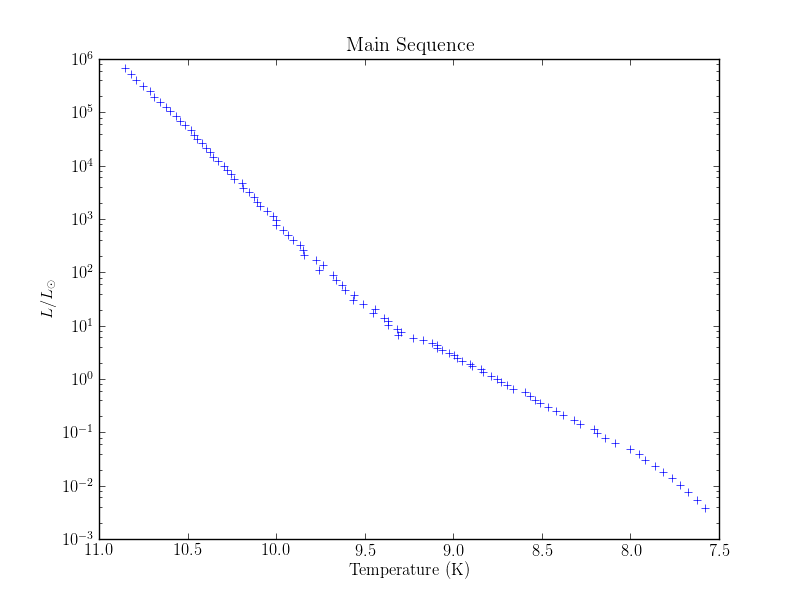
\includegraphics[scale=0.7]{plots/main_sequence/ms.png}
\caption{HR diagram of 100 main sequence stars with central temperatures ranging from 5$\times$10$^6$ K to 3.5$\times$10$^7$ K}
\label{ms}
\end{figure}

As expected, an increase in surface temperature increases luminosity. This plot agrees with the theory. 

The following two figures, figures \ref{LvM} and \ref{RvM}, are the $L/L_\odot$ vs $M/M_\odot$ and $R/R_\odot$ vs $M/M_\odot$ plots of 100 main sequence stars with central temperatures ranging from 5$\times$10$^6$ K to 3.5$\times$10$^7$ K respectively. Also shown in each plot are the empirical expressions found in the text, p. 330 \cite{text}.

\begin{figure}[h!]
\centering
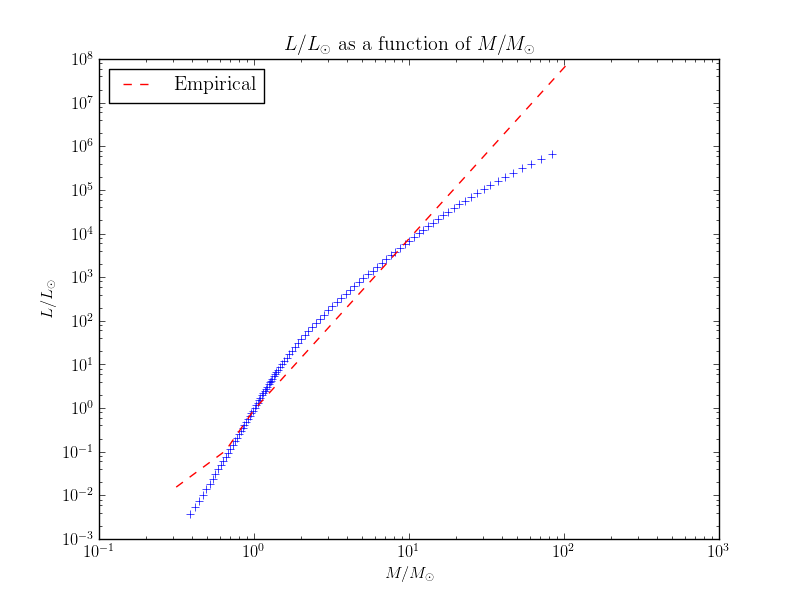
\includegraphics[scale=0.6]{plots/main_sequence/LvM.png}
\caption{luminosity vs mass plot of 100 main sequence stars with central temperatures ranging from 5$\times$10$^6$ K to 3.5$\times$10$^7$ K}
\label{LvM}
\end{figure}

\begin{figure}[h!]
\centering
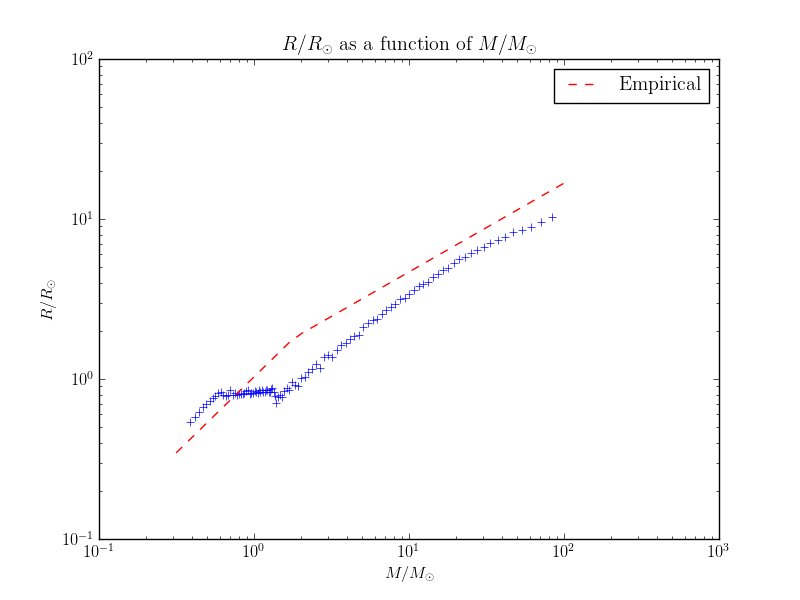
\includegraphics[scale=0.6]{plots/main_sequence/RvM.png}
\caption{radius vs mass plot of 100 main sequence stars with central temperatures ranging from 5$\times$10$^6$ K to 3.5$\times$10$^7$ K}
\label{RvM}
\end{figure}

The calculated plots agree with the empirical expressions well. There is an interesting feature in the $R/R_\odot$ vs $M/M_\odot$ plot where the stars' radius seem to remain constant as you increase mass in a region near where the empirical expression changes, but other than this feature, the plots seem to agree.\\

\newpage
\null
\newpage

\section{Stellar Structure}

Two stars, one of mass 0.709$M_\odot$ and another of mass 35$M_\odot$, were used to compare stellar structure. The following table 2 details each stars' surface temperature, central density, radius, mass, and luminosity.

\begin{table}[h!]
\begin{center}
\begin{tabular}{| r | l | l |}
\hline
 & Star 1 & Star 2 \\
\hline
Central Temperature & 9$\times$10$^6$ K & 3.5$\times$10$^7$ K \\
\hline
Surface Temperature & 3795 K & 41885 K \\
\hline
Central Density & 74238 kg/m$^3$ & 1237 kg/m$^3$ \\
\hline
Radius & 0.81$R_\odot$ & 7.08$R_\odot$ \\
\hline
Mass & 0.709$M_\odot$ & 35$M_\odot$ \\
\hline
Luminosity & 0.122$L_\odot$ & 1.4$\times$10$^5L_\odot$ \\
\hline
\end{tabular}
\caption{Butcher tableau of RKF45}
\end{center}
\end{table} 

Their features such as $\rho$, $T$, $M$, $L$, $P$, $dL/dr$, and $\kappa$ were plotted as functions of $r/R_*$, as well as their partial pressures, luminosities, opacities, and the dlogP/dlogT, as shown in the below figures. \\

\begin{figure}[h!]
\centering
\begin{subfigure}{.5\textwidth}
  \centering
  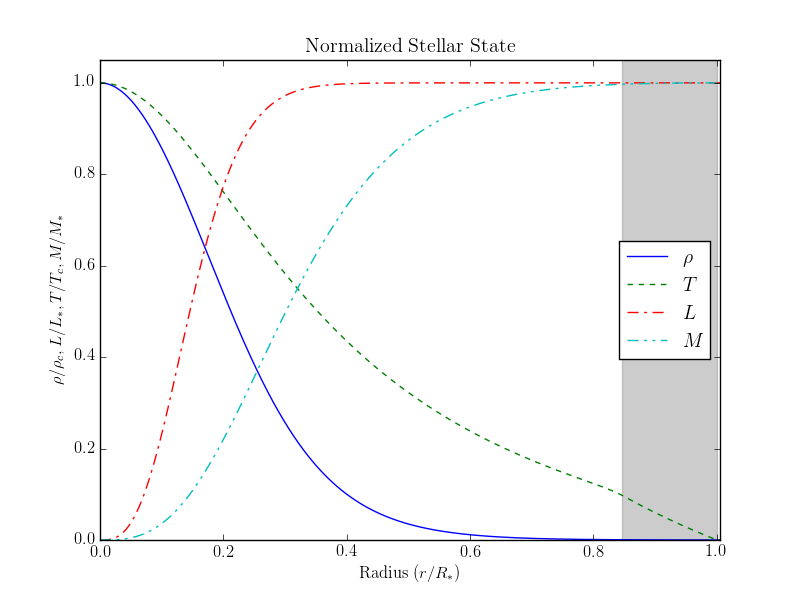
\includegraphics[scale=0.5]{plots/star_comp-_X-0.73,Y-0.25,Z-0.02__Tc-9000000.0/stellar_state.png}
  \caption{Stellar structure plots of star with mass 0.709$M_\odot$}
  \label{fig:sssmall}
\end{subfigure}%
\begin{subfigure}{.5\textwidth}
  \centering
  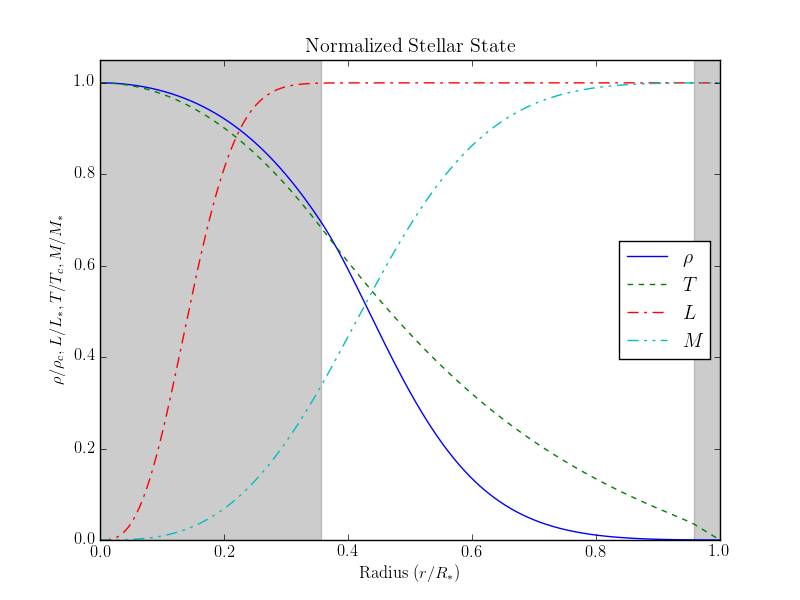
\includegraphics[scale=0.5]{plots/star_comp-_X-0.73,Y-0.25,Z-0.02__Tc-33000000.0/stellar_state.png}
  \caption{Stellar structure plots of star with mass 35$M_\odot$}
  \label{fig:ssbig}
\end{subfigure}
\caption{Stellar structure plots of both stars}
\label{fig:ss}
\end{figure}

\begin{figure}[h!]
\centering
\begin{subfigure}{.5\textwidth}
  \centering
  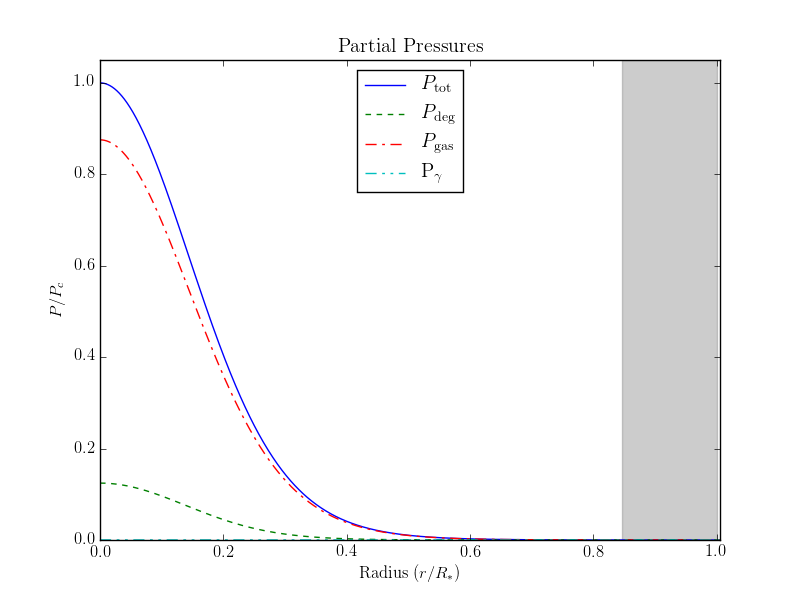
\includegraphics[scale=0.5]{plots/star_comp-_X-0.73,Y-0.25,Z-0.02__Tc-9000000.0/partial_pressure.png}
  \caption{Partial pressure plot of star with mass 0.709$M_\odot$}
  \label{fig:ppsmall}
\end{subfigure}%
\begin{subfigure}{.5\textwidth}
  \centering
  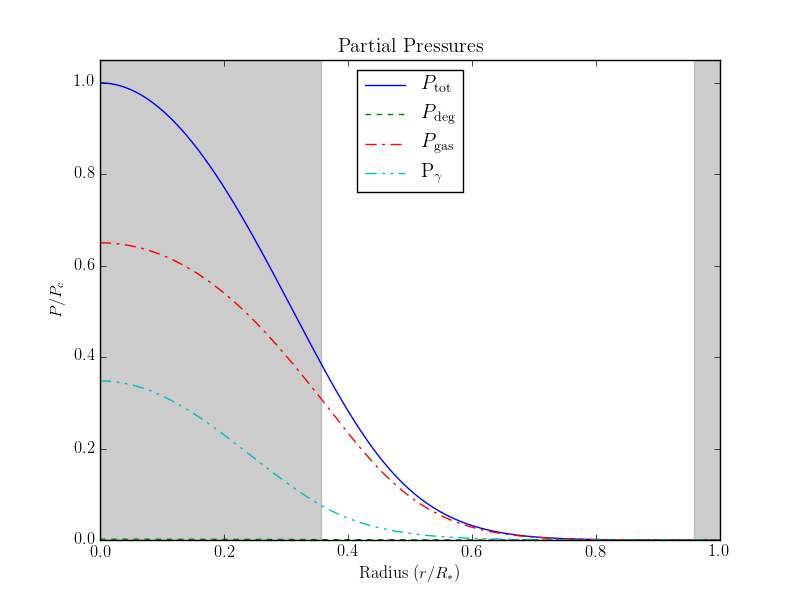
\includegraphics[scale=0.5]{plots/star_comp-_X-0.73,Y-0.25,Z-0.02__Tc-33000000.0/partial_pressure.png}
  \caption{Partial pressure plot of star with mass 35$M_\odot$}
  \label{fig:ppbig}
\end{subfigure}
\caption{Partial pressure plots of both stars}
\label{fig:pp}
\end{figure}

\begin{figure}[h!]
\centering
\begin{subfigure}{.5\textwidth}
  \centering
  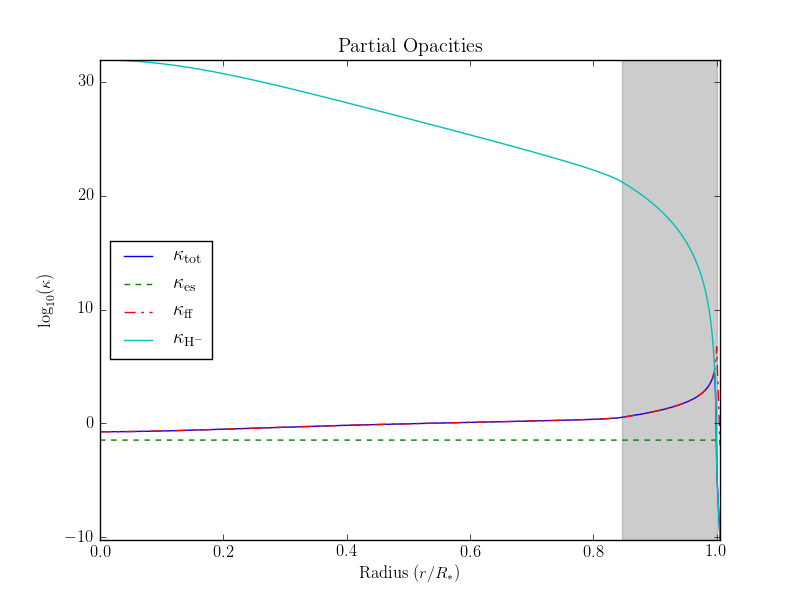
\includegraphics[scale=0.5]{plots/star_comp-_X-0.73,Y-0.25,Z-0.02__Tc-9000000.0/partial_opacity.png}
  \caption{Partial opacity plot of star with mass 0.709$M_\odot$}
  \label{fig:posmall}
\end{subfigure}%
\begin{subfigure}{.5\textwidth}
  \centering
  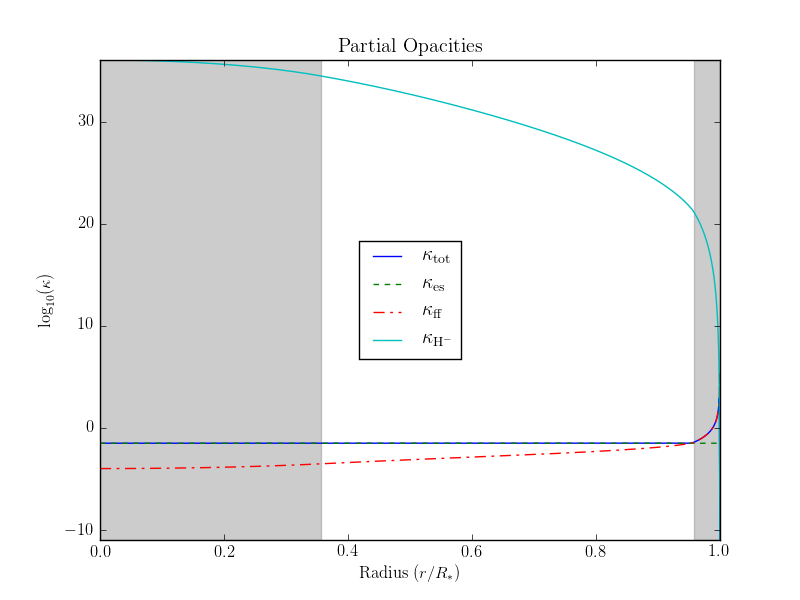
\includegraphics[scale=0.5]{plots/star_comp-_X-0.73,Y-0.25,Z-0.02__Tc-33000000.0/partial_opacity.png}
  \caption{Partial opacity plot of star with mass 35$M_\odot$}
  \label{fig:pobig}
\end{subfigure}
\caption{Partial opacity plots of both stars}
\label{fig:po}
\end{figure}

\begin{figure}[h!]
\centering
\begin{subfigure}{.5\textwidth}
  \centering
  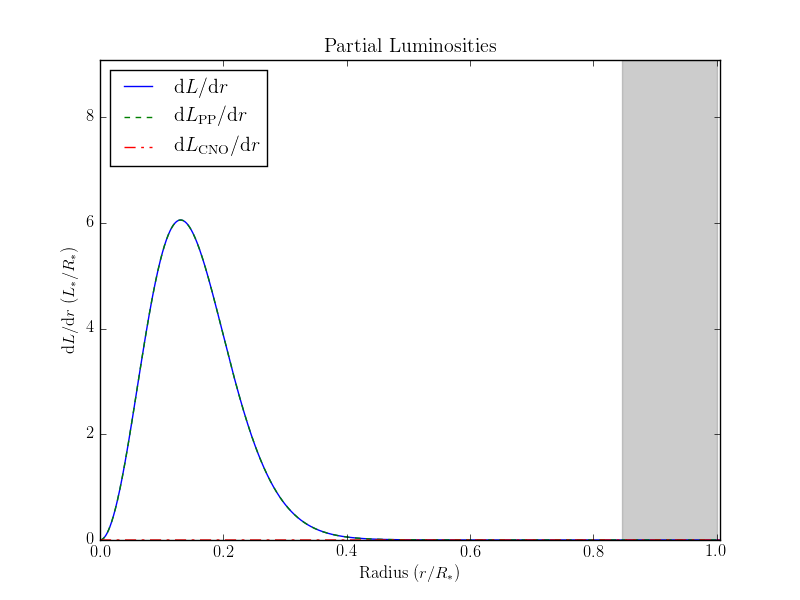
\includegraphics[scale=0.5]{plots/star_comp-_X-0.73,Y-0.25,Z-0.02__Tc-9000000.0/partial_lumin.png}
  \caption{Partial luminosity plot of star with mass 0.709$M_\odot$}
  \label{fig:plsmall}
\end{subfigure}%
\begin{subfigure}{.5\textwidth}
  \centering
  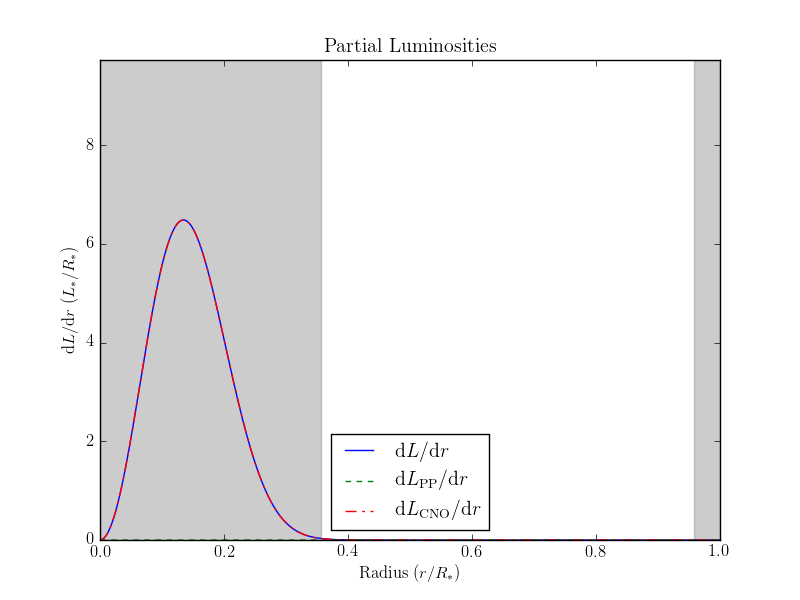
\includegraphics[scale=0.5]{plots/star_comp-_X-0.73,Y-0.25,Z-0.02__Tc-33000000.0/partial_lumin.png}
  \caption{Partial luminosity plot of star with mass 35$M_\odot$}
  \label{fig:plbig}
\end{subfigure}
\caption{Partial luminosity plots of both stars}
\label{fig:pl}
\end{figure}

\begin{figure}[h!]
\centering
\begin{subfigure}{.5\textwidth}
  \centering
  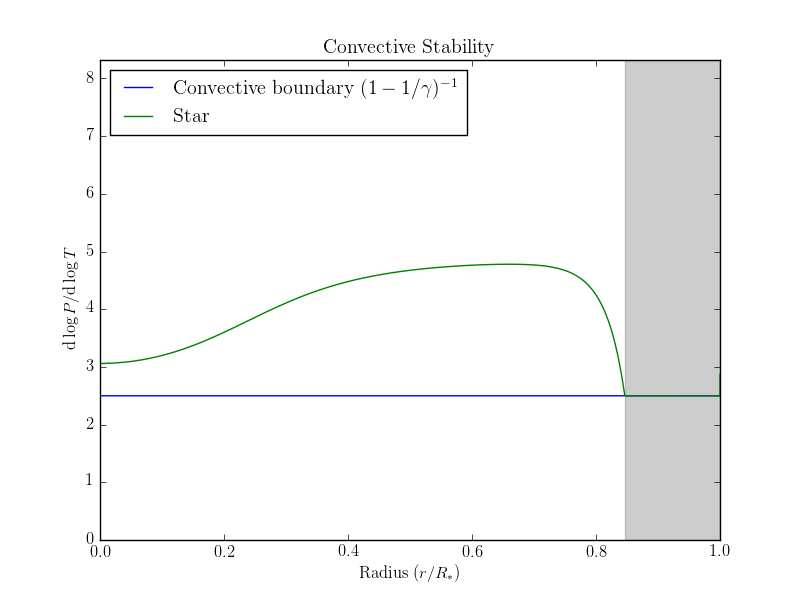
\includegraphics[scale=0.5]{plots/star_comp-_X-0.73,Y-0.25,Z-0.02__Tc-9000000.0/dlogP_dlogT.png}
  \caption{Convective stability plot of star with mass 0.709$M_\odot$}
  \label{fig:cssmall}
\end{subfigure}%
\begin{subfigure}{.5\textwidth}
  \centering
  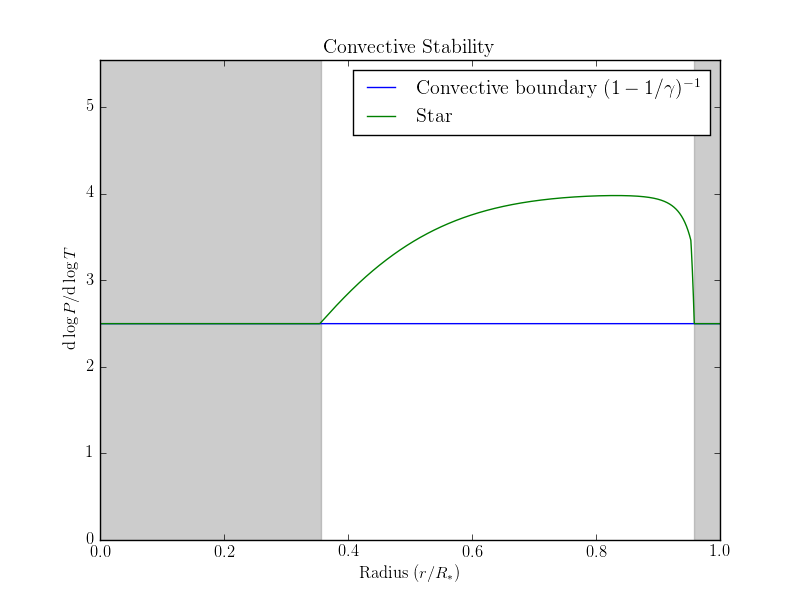
\includegraphics[scale=0.5]{plots/star_comp-_X-0.73,Y-0.25,Z-0.02__Tc-33000000.0/dlogP_dlogT.png}
  \caption{Convective stability plot of star with mass 35$M_\odot$}
  \label{fig:csbig}
\end{subfigure}
\caption{Convective stability plots of both stars}
\label{fig:cs}
\end{figure}

\newpage
\null
\newpage

An interesting feature to note is that the convective zone in the 0.709 solar mass star is entirely at the surface of the star, taking about 15\% of the total radius of the star, while the rest of the star is radiative. However, the 34 solar mass star has a large convective zone at the center of the star that takes up about 35\% of the radius, and another convective zone at the surface taking about 5\% of the radius, with a radiative zone in between. This large convective zone at the center appears due to the fact that photon gas pressure is contributory to the total pressure, and it scales with T$^4$, forcing both terms in the temperature gradient to scale with T$^3$, allowing the convective term to become the flatter of the two and drive convection. The photon gas pressure in the 0.709 mass star is not as contributory until about the last 15\% of the star's radius, which is why it doesn't have a convective zone until then.

Looking at figure 7, in the 0.709 solar mass star, the PP chain dominates over the CNO cycle. However, for the 34 solar mass star, the CNO cycle dominates over the PP chain. This is because the CNO cycle only kicks in at approximately 1.7$\times$10$^7$ K, and since the central temperature of the lower mass star is lower than that at 9$\times$10$^6$ K, its temperature is too low for the CNO cycle to kick in. The 34 solar mass star has a temperature of 3.5$\times$10$^7$ K, which is higher than the requirement for the CNO cycle to kick in, and maintains a high enough temperature throughout its central convective region for the CNO cycle to dominate. The CNO cycle dominates over the PP chain for the large mass star because the CNO cycle energy generation rate scales with T$^19.9$, whereas the PP chain energy generation rate scales with only T$^4$, so a higher temperature means the CNO cycle energy generation rate increases faster than the PP chain, resulting in its domination.

Looking at figure 6, in the 0.709 solar mass star, the free-free scattering opacity dominates over the electron scattering opacity until it reaches the surface of the star where the H$^-$ opacity takes over and drives the opacity down. However, for the 34 solar mass star, the electron scattering opacity dominates over the free-free scattering opacity throughout most of the star until it reaches the surface convective zone where the free-free scattering opacity takes over, followed by the H$^-$ opacity near the surface of the star. The larger mass star is mostly dominated by electron scattering opacity because the equation for total opacity is:

\begin{equation}
\kappa(\rho, T) = \left[\frac{1}{\kappa_{H^-}} + \frac{1}{\text{max}(\kappa_{es}, \kappa_{ff})}\right]^{-1}
\end{equation} \label{f_rho}

with each components being:

\begin{equation}
\kappa_{es} = 0.02(1+X)\text{m}^2\text{/kg}
\end{equation} \label{f_rho}
\begin{equation}
\kappa_{ff} = 1.0\times10^{24}(Z+0.0001)\rho_{3}^{0.7} T^{-3.5}\text{m}^2\text{/kg}
\end{equation} \label{f_rho}
\begin{equation}
\kappa_{H^-} = 2.5\times10^{-32}(Z/0.02)\rho_{3}^{0.5} T^{9}\text{m}^2\text{/kg}
\end{equation} \label{f_rho}

\cite{manual}Note that free-free scattering opacity scales with T$^-3.5$ (the higher the temperature, the smaller it's opacity) whereas electron scattering opacity only depends on X (the mass fraction of hydrogen), and so remains flat throughout the star no matter the temperature or density. Also note that the total opacity is driven by the maximum of either electron scattering or free-free scattering, and is the sum of the inverse of either of those two and the H$^-$ opacity. For the large mass star, the temperature is high enough for the free-free scattering opacity to fall below the electron scattering opacity, allowing the electron scattering opacity to dominate throughout most of the star, until the temperature decreases low enough for the free-free scattering opacity to rise above the electron scattering opacity and take over. The smaller mass star doesn't have a high enough temperature for the free-free scattering opacity to fall below the electron scattering opacity, and so it remains dominated by the free-free scattering opacity throughout most of the star. H$^-$ opacity scales with T$^9$, and so remains high throughout most of both of the stars, contributing not much to the total opacity, until the temperature drops enough for it to drop below the free-free scattering opacity near the surface of the star and take over all the way to the surface.

\newpage

\section{Appendix}\label{appendix}
stellar\_generatory.py:
\lstinputlisting[language=Python]{StellarModellingMetallicity/code/stellar_generator.py}

stellar\_plotter.py:
\lstinputlisting[language=Python]{StellarModellingMetallicity/code/stellar_plotter.py}

main\_sequence.py:
\lstinputlisting[language=Python]{StellarModellingMetallicity/code/main_sequence.py}

rkf.py:
\lstinputlisting[language=Python]{StellarModellingMetallicity/code/rkf.py}

adaptive\_bisection.py:
\lstinputlisting[language=Python]{StellarModellingMetallicity/code/adaptive_bisection.py}

\newpage

\begin{thebibliography}{9}

	\bibitem{DE} Hairer, E., N{\o}rsett, S. P., \& Wanner, G. (1987). \textit{Solving ordinary differential equations}. Berlin: Springer-Verlag.
	
	\bibitem{manual} \textit{Physics 375 Final Project}. Waterloo (ON): University of Waterloo.
	
	\bibitem{text} Ryden, B. S., \& Peterson, B. M. (2010). \textit{Foundations of Astrophysics}. San Francisco: Addison-Wesley.
	
\end{thebibliography}

\end{document}
